\documentclass[a4paper, titlepage]{article}

% For equations
\usepackage{amsmath}

% For including figures
\usepackage{graphicx}
\usepackage{float}

% Bibiliography setup
\usepackage[square]{natbib}
\bibliographystyle{agsm}
\usepackage[nottoc]{tocbibind}

% For typesetting matlab
\usepackage{listings}
\usepackage{color} %red, green, blue, yellow, cyan, magenta, black, white
\definecolor{mygreen}{RGB}{28,172,0} % color values Red, Green, Blue
\definecolor{mylilas}{RGB}{170,55,241}

\lstset{language=Matlab,%
    basicstyle=\small,
    breaklines=true,%
    frame = single,
    morekeywords={matlab2tikz},
    keywordstyle=\color{blue},%
    morekeywords=[2]{1}, keywordstyle=[2]{\color{black}},
    identifierstyle=\color{black},%
    stringstyle=\color{mylilas},
    commentstyle=\color{mygreen},%
    showstringspaces=false,
    numbers=left,%
    numberstyle={\tiny \color{black}},% size of the numbers
    numbersep=9pt, % this defines how far the numbers are from the text
    emph=[1]{for,end,break},emphstyle=[1]\color{red}, %some words to emphasise
    %emph=[2]{word1,word2}, emphstyle=[2]{style},    
}


\title{Laboratory Work 2\\
System description and analysis\\
\large EEA004}
\author{Dan Thilderkvist, Philip Gutierrez}

\begin{document}

\maketitle

\section{Introduction}
In this laboratory work an unstable system is to be analyzed.
The ball and beam experiment setup, figure X, will serve the purpose as the unstable system.
The ball and beam setup is controlled by the DC motor torque and the measured output is the position of the ball on the beam.
In table X, the physical quantities of the system are listed.

\begin{figure}[h!]
\center
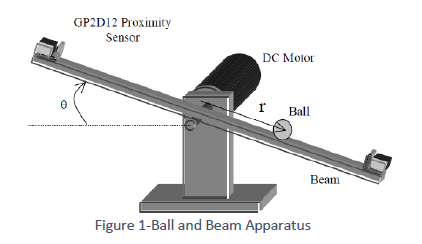
\includegraphics[scale=0.8]{../figures/ballAndBeam.png}
\caption{The ball and beam experiment setup and the system variables $\theta$ and $r$.}
\label{fig:ballAndBeam}
\end{figure}

\begin{table}[h!]
\centering
 \begin{tabular}{||c c c||} 
 \hline
 Abbreviation & Description & Value \\ [0.5ex] 
 \hline\hline
 $m$ & mass of the ball & 0.11 kg \\ 
 $R$ & radius of the ball & 0.015 m \\
 $M$ & mass of the beam & 1 kg \\
 $g$ & gravitational acceleration & 9.8 m/s\textsuperscript{2} \\
 $L$ & length of the beam & 1.0 m \\
 $J_R$ & ball's moment of inertia & 1e-5 kgm\textsuperscript{2} \\
 $J$ & beam's moment of inertia & 2e-3 kgm\textsuperscript{2} \\
 $r$ & ball position coordinate & \\
 $\theta$ & beam angle coordinate &  \\ [1ex] 
 \hline
 \end{tabular}
 \caption{The quantities of the ball and beam system used in the exercise.}
 \label{tab:quantities}
\end{table}


\section{Theory}

\section{Method}

\section{Results}

\section{Discussion}

\section{Conclusion}

\clearpage
\bibliography{reference}

\clearpage
\appendix

\section{Example Section}
This is an example reference \citep{glad00}.

\begin{figure}[h!]
\center
\includegraphics[scale=0.8]{../code/figures/exampleFigure.png}
\caption{Example caption.}
\label{fig:exampleLable}
\end{figure}

\lstinputlisting{../code/exampleCode.m}

\end{document}